\section{Data Acquisition}
\label{sec:chap_slam_data_acquisition}

In the following section, we first describe the robotic platform and sensors used to gather our place recognition dataset. We then describe in more details the dataset acquisition procedure and the resulting data.


\subsection{Robotic Platform}
\label{ssec:chap_slam_platform}

The Husky A200 is a medium size (\SI{990 x 670 x 390}{\milli\meter}) \gls*{ugv} developed by \cite{ClearpathWeb}. It is a rugged robot designed for all terrain conditions and it uses a differential-drive skid steer, allowing easy control and in-place turns. The maximum speed of the vehicle is \SI{1}{\meter\per\second} and the maximum payload capability is \SI{75}{\kilo\gram}. This robotic platform is well suited for our needs, because it can move in forests and carry the required equipment. Our platform is shown in Figure~\ref{fig:chap_slam_husky} and details about the available devices are presented in Table~\ref{tab:husky_devices}. 

\begin{figure}[H]
    \centering
    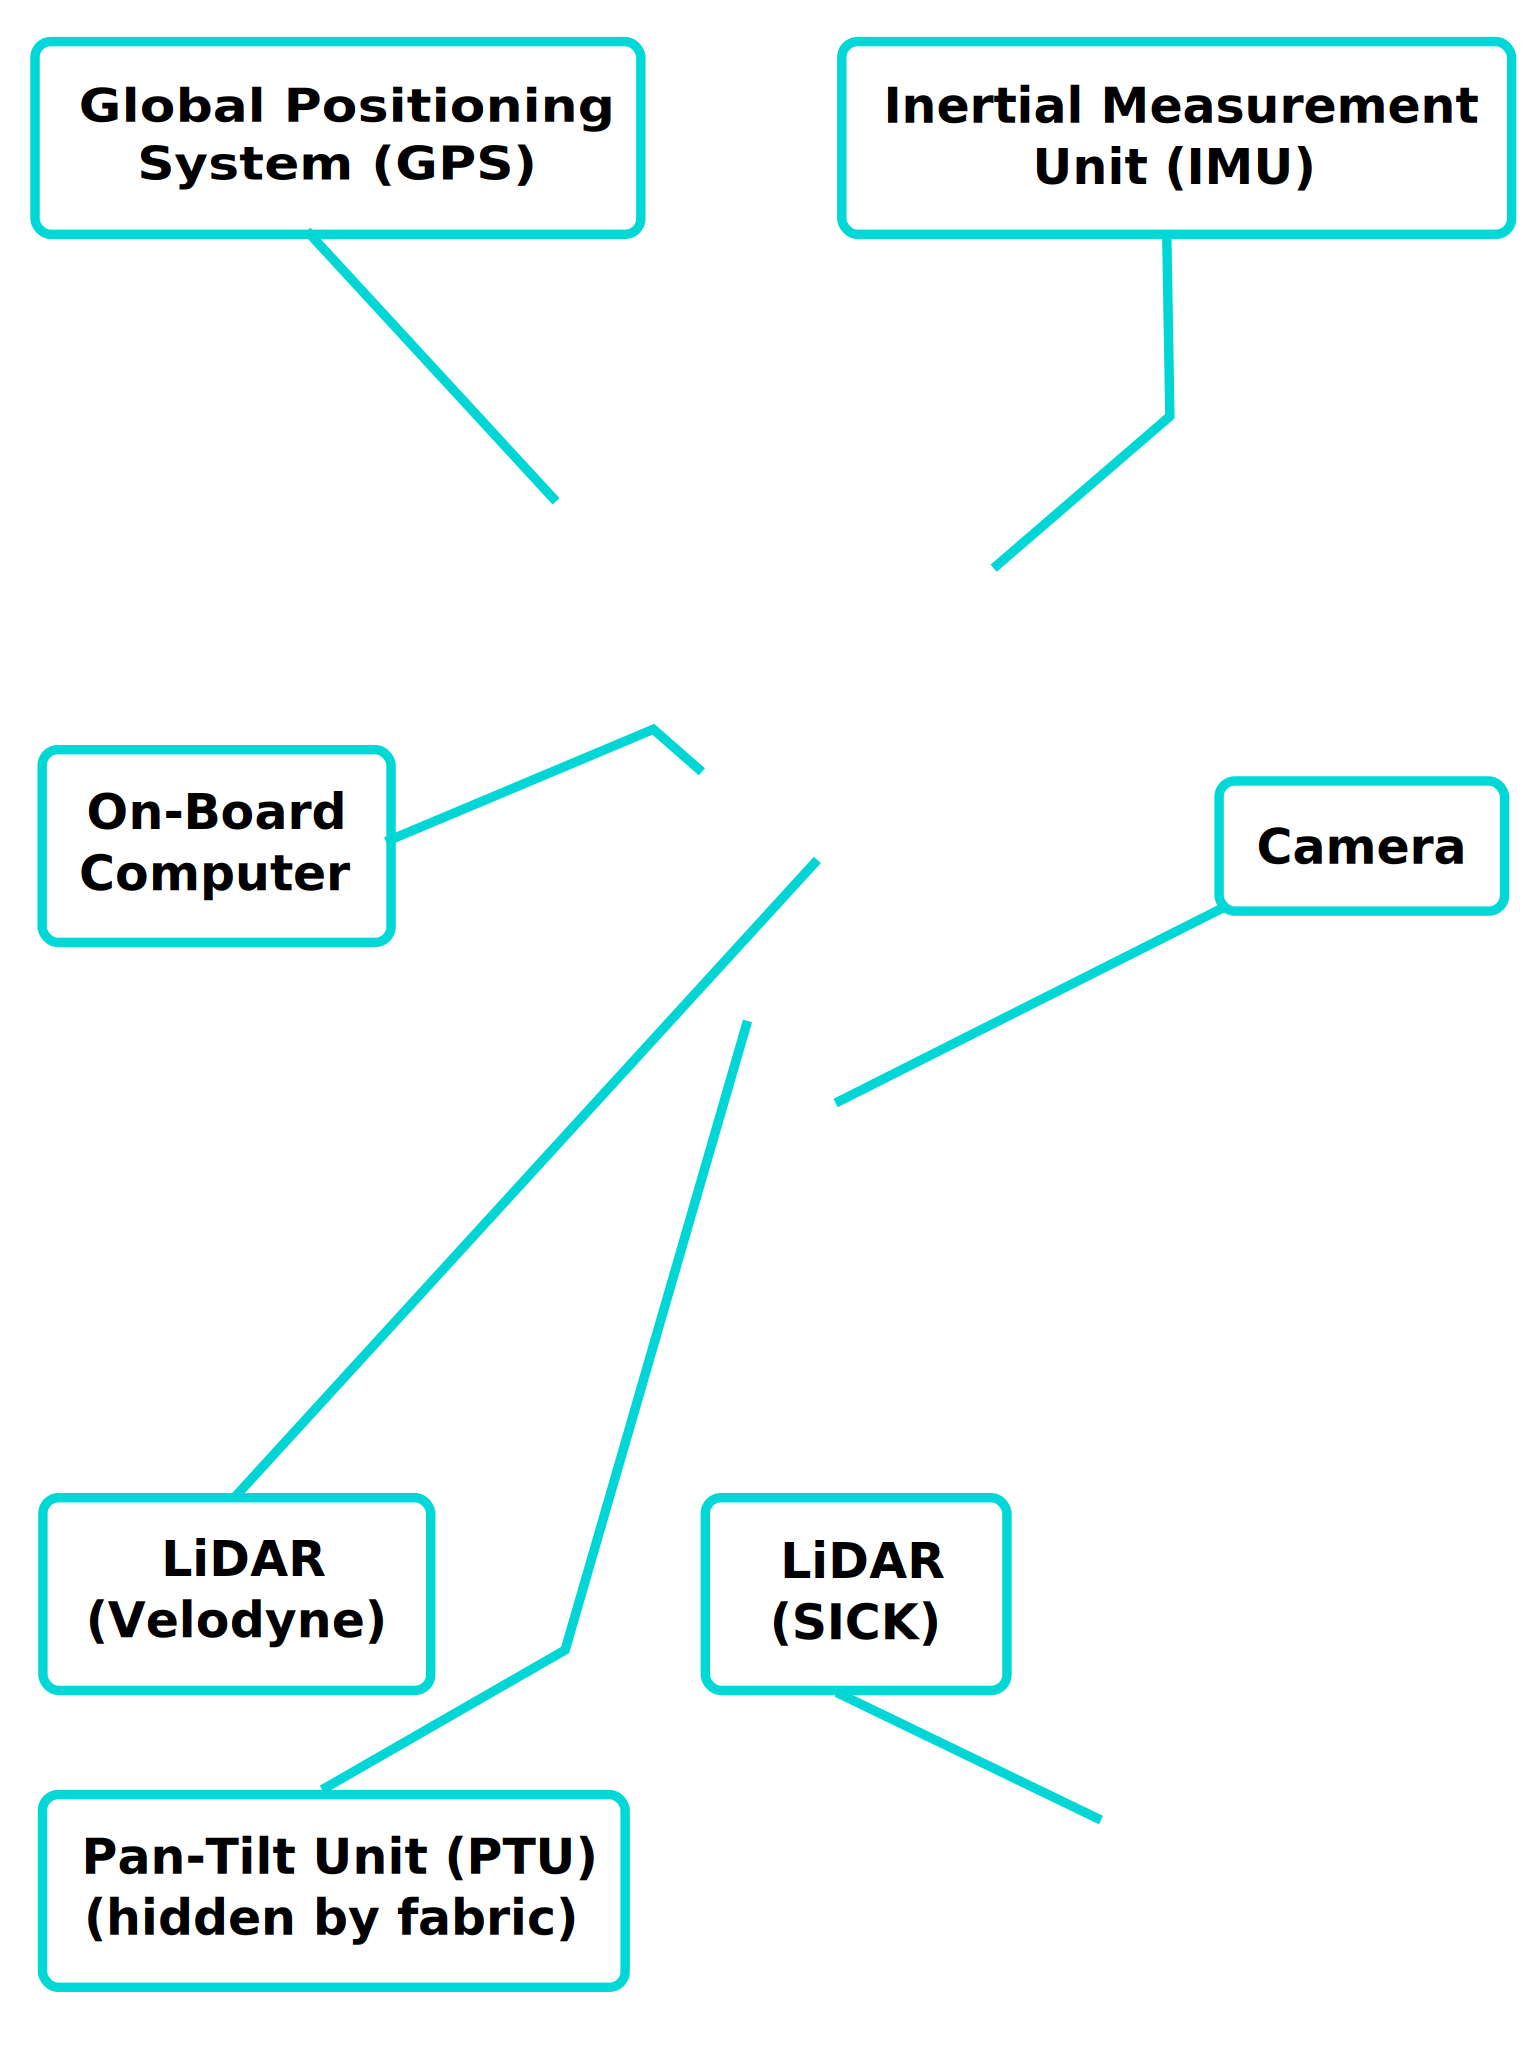
\includegraphics[width=0.98\linewidth]{img/chap_slam/husky_labelled.png}
    \caption[Our robotic platform (Husky A200) and the devices used for data acquisition.]{Our robotic platform (Husky A200) and the devices used for data acquisition. The SICK \gls*{lidar} is not mounted, but instead is shown on the bottom right corner of the figure. Note that the \gls*{ptu} is hidden by a cover and the on-board computer is mostly occluded by the Velodyne \gls*{lidar}.}
    \label{fig:chap_slam_husky}
\end{figure}

\begin{table}[H]
    \centering
    \begin{tabular}{@{}llll@{}}
        \toprule
        \textbf{Device} & \textbf{Manufacturer}       & \textbf{Model}  & \textbf{Use}                          \\ \hline
        Computer        & --                          & --              & Data acquisition/synchronisation      \\
        Gateway         & Microhard System Inc.       & VIP2400         & Network and Wi-Fi communication       \\
        Gamepad         & Logitech                    & F710            & Remote control of the robot movements \\
        \gls*{lidar}    & Velodyne                    & HDL-32E         & Point cloud acquisition               \\
        \gls*{lidar}    & SICK                        & LMS151          & Point cloud acquisition               \\
        \gls*{ptu}      & FLIR Motion Control Systems & D46-17          & Rotate the SICK \gls*{lidar}          \\
        \gls*{imu}      & ChRobotics                  & UM6             & Odometry                              \\
        Camera          & Axis                        & M1013           & Visual reference                      \\
        \gls*{gps}      & NovAtel                     & SMART6          & Not used                              \\
        \bottomrule
    \end{tabular}
    \caption[List of devices available on the Husky A200 and their use in our experiments.]{List of devices available on the Husky A200 and their use in our experiments. Note that both \gls*{lidar}s were never mounted at the same time.}
    \label{tab:husky_devices}
\end{table}

The on-board computer (2.4 GHz Intel i5-520M) is an essential element of our experiments, as it connects all devices, acts as a control interface for the robot and stores the acquired data. The computer does not provide a \gls*{gui}, but is connected to the gateway that broadcasts a WiFi network, allowing \gls*{ssh} communication. The platform is also equipped with a wireless gamepad, which enables manual control of the movements of the robot. Point clouds acquisition is possible using either the SICK LMS151 or the Velodyne HDL-32E. The selected sensor is mounted on the \gls*{ptu}, which remains fixed for the Velodyne, but is rotated with the SICK to merge multiple \gls*{2d} scans into a single \gls*{3d} point cloud. Section~\ref{ssec:chap_slam_platform} gives more details about the resulting point clouds for each sensor.

The sensors described above are essential for our place recognition research, but we also use the wheel encoders along with the \gls*{imu} for odometry estimation and the camera for visual reference of the dataset. Note that we do not use the \gls*{gps}, as it is not reliable in forests. 


\subsection{Dataset Description}
\label{ssec:chap_slam_platform}

Data acquisition was performed using \gls*{ros}, a set of software libraries and tools created to simplify the development of robotics applications. It provides, out of the box, all drivers for the Husky and our sensors. Its data publishing system provides timestamps that allow easy synchronization between sensors. The recording tool (rosbag) was used to create our datasets, with data processing performed \textit{a posteriori}.

We produced datasets in two different areas of the Laval University campus. An aerial overview of the path followed by the robot at these two locations is presented in Figure~\ref{fig:chap_slam_path}.

The first site was chosen for its more structured nature and is located between the Alexandre-Vachon and the Adrien-Pouliot buildings. This environment is mostly open, the terrain is smooth and flat and the site contains man-made objects such as buildings, stairs or tables. Examples of pictures acquired by the robot on this site are presented in Figure~\ref{fig:slam_view_building1} and~\ref{fig:slam_view_building2}. This dataset closely resembles the kind of data on which several place recognition algorithms are typically tested on (e.g. Freiburg Campus 360 degree 3D scans~\citep{FreiburgDataset}, Robotic 3D Scan Repository~\citep{Datasets}).

The second site, chosen for its unstructured nature, is located in a wooded area, also on the Laval University campus. The dataset path starts on a pedestrian walkway, but after its second turn (of approximately \SI{330}{\degree}), it continues for around \SI{100}{\meter} in rougher terrain. This forested environment presents multiple small structures and significant of occlusions. Figure~\ref{fig:slam_view_forest1} and Figure~\ref{fig:slam_view_forest2} show pictures from the robot camera at this location. This dataset will allow us to better understand the influence of a less structured environment on the place recognition algorithm. In particular, the absence of large flat surfaces and corners typical of buildings, as well as the closeness of the space, will be challenging for place recognition algorithms.

\begin{figure}[H]
    \centering
    \subfloat[]{\label{fig:path_overview}}{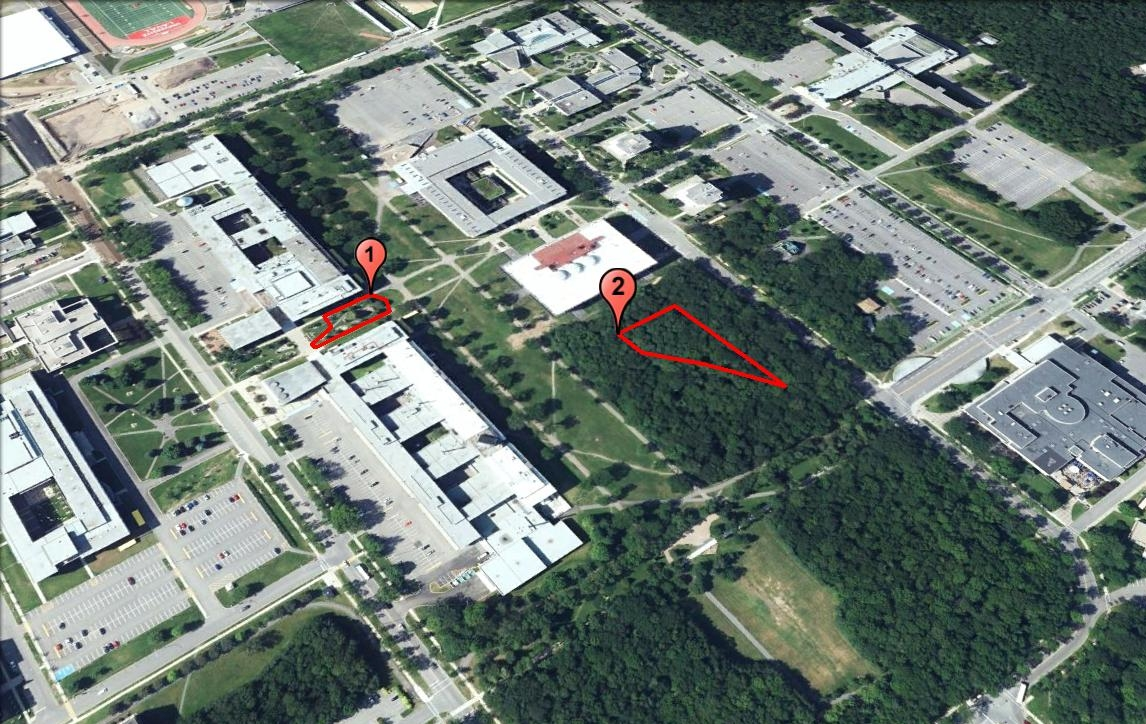
\includegraphics[width=0.995\linewidth]{img/chap_slam/paths.jpg}}\\ \vspace{3mm}
    \subfloat[]{\label{fig:path_building}}{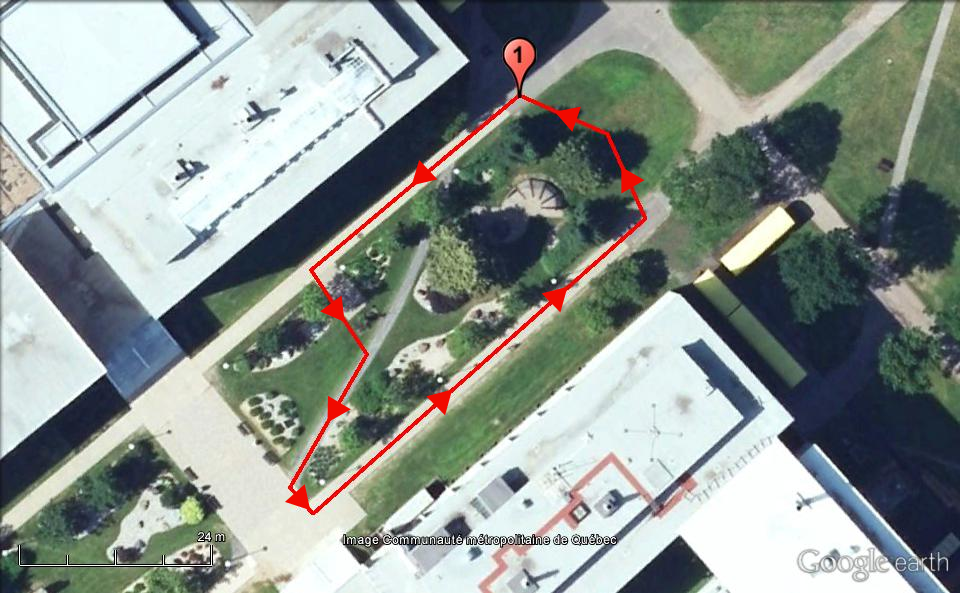
\includegraphics[width=0.485\linewidth]{img/chap_slam/path_building_arrow.png}} \hspace{2mm}
    \subfloat[]{\label{fig:path_forest}}{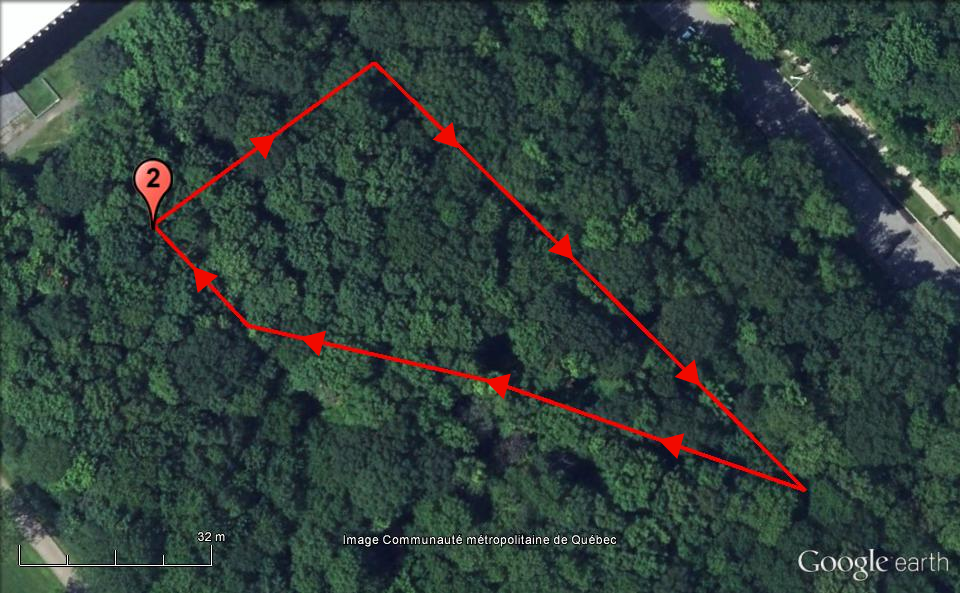
\includegraphics[width=0.485\linewidth]{img/chap_slam/path_forest_arrow.png}}
    \caption[Partial aerial view of the Laval University campus including the two approximate paths followed by the robot for data acquisition.]{\protect\subref{fig:path_overview} Partial aerial view of the Laval University campus including the two approximate paths followed by the robot for data acquisition. \protect\subref{fig:path_building} Zoomed view of the path followed (counterclockwise from tag 1) in a structured environment. The length of this path is approximately \SI{160}{\meter}. \protect\subref{fig:path_forest} Zoomed view of the path followed (clockwise from tag 2) to create the unstructured datasets. The length of this path is approximately \SI{275}{\meter}. Images source: Google Earth, (2015)}
    \label{fig:chap_slam_path}
\end{figure}

\begin{figure}[H]
    \centering
    \subfloat[]{\label{fig:slam_view_building1}}{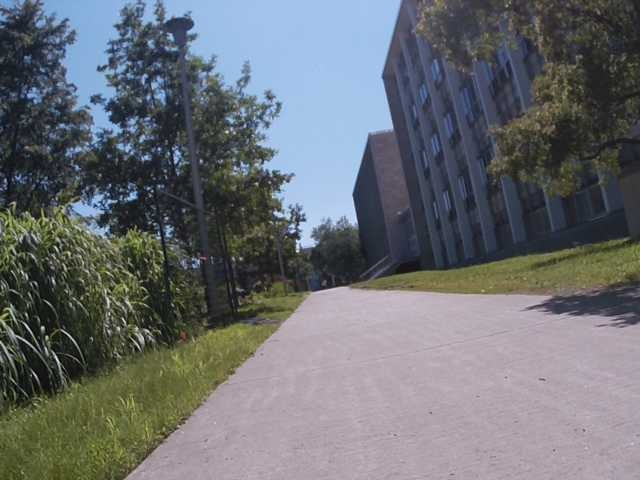
\includegraphics[width=0.47\linewidth]{img/chap_slam/building_view1.jpg}} \hspace{2mm}
    \subfloat[]{\label{fig:slam_view_building2}}{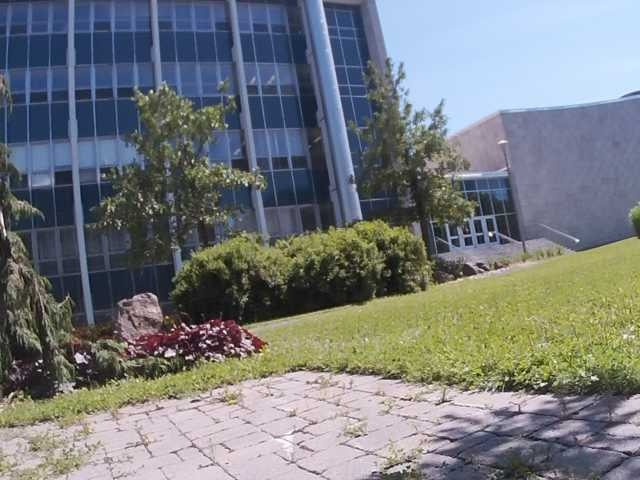
\includegraphics[width=0.47\linewidth]{img/chap_slam/building_view2.jpg}}
    \subfloat[]{\label{fig:slam_view_forest1}}{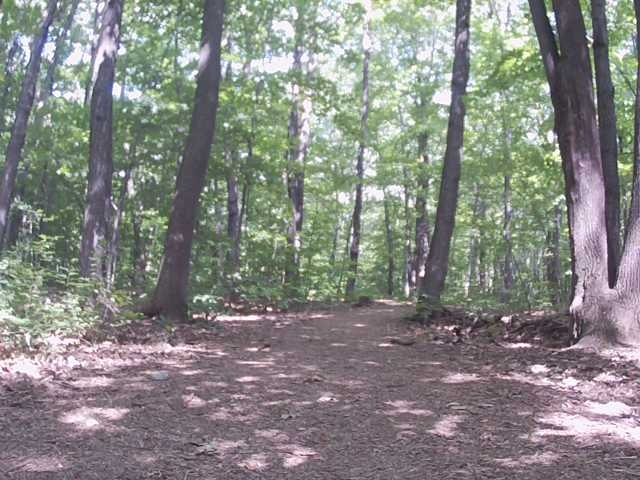
\includegraphics[width=0.47\linewidth]{img/chap_slam/forest_view1.jpg}} \hspace{2mm}
    \subfloat[]{\label{fig:slam_view_forest2}}{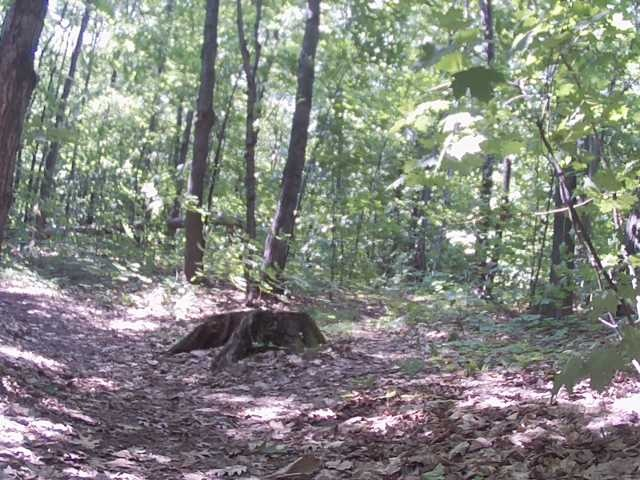
\includegraphics[width=0.47\linewidth]{img/chap_slam/forest_view2.jpg}}
    \caption[Images from the \gls*{ugv} camera during the acquisition of the two datasets.]{Images from the \gls*{ugv} camera during the acquisition of the structured dataset \protect\subref{fig:slam_view_building1} \protect\subref{fig:slam_view_building2} and the unstructured dataset \protect\subref{fig:slam_view_forest1} \protect\subref{fig:slam_view_forest2}. Note that the images are at an angle for the unstructured dataset, because the camera was not aligned with the robot during acquistion.}
    \label{fig:slam_views}
\end{figure}

To evaluate the impact of the sensor used and data associated with it, we will use the SICK and the Velodyne, for which you can find details in Table~\ref{tab:slam_sensor_resolution}.

The SICK is a \gls*{2d} \gls*{lidar} with a scanning angle of \SI{270}{\degree}, a resolution of \SI{0.5}{\degree} and an acquisition frequency of \SI{50}{\hertz}. This sensor was placed on the \gls*{ptu} so that the blind spot faced downward. During acquisition, it was rotated around the vertical axis (pan) at a speed of \SI{14.32}{\degree\per\second} for half a turn, while the vehicle was stationary. This procedure allowed the acquisition of 628 \gls*{2d} scans of \SI{540}{\points}, later merged into a single \gls*{3d} point cloud. To create the dataset using the SICK, the robot was stopped at regular interval on the established path to acquire scans.

The Velodyne, for its part, directly allows \gls*{3d} point cloud acquisition by spinning 32 lasers around its vertical axis. These lasers are evenly distributed between \SI{-30.67}{\degree} and \SI{10.67}{\degree} relative to the horizontal plane. According to the Velodyne datasheet \citep{VelodyneDatasheet}, the device acquires approximately \SI{700000}{\points\per\second} and publishes at \SI{10}{\hertz}, therefore creating point clouds of \SI{70000}{\points}. Note that these point counts are variable as the rotation speed can change slightly and the use of the \gls*{udp} can lead to some loss of points. Regarding the dataset acquisition, the robot was driven at a constant speed (\SI{0.3}{\meter\per\second}) and performed data acquisition simultaneously. In order to obtain a quantity of scans similar to that produced with the SICK, only one out of 80 scans was used to create the final dataset.

Table~\ref{tab:slam_sensor_resolution} summarizes information about the sensors resolution and \gls*{fov}, while Table~\ref{tab:slam_datasets} provides a name for later references and additional information about each of our datasets.

\begin{table}[H]
    \centering
    \begin{tabular}{@{}lrrrrr@{}}
        \toprule
        \makecell[lc]{\textbf{Sensor}}& \makecell[cc]{\textbf{Horizontal}\\\textbf{resolution}} & \makecell[cc]{\textbf{Vertical}\\\textbf{resolution}} & \makecell[cc]{\textbf{Minimum}\\\textbf{angle}} & \makecell[cc]{\textbf{Maximum}\\\textbf{angle}} & \makecell[cc]{\textbf{Point}\\\textbf{counts}} \\
        \hline
        SICK LMS151      & \SI{0.57}{\degree} & \SI{0.5}{\degree}  & \SI{-45.00}{\degree}  & \SI{90.00}{\degree}  & 339120 \\
        Velodyne HDL-32E & \SI{0.16}{\degree} & \SI{1.33}{\degree} & \SI{-30.68}{\degree}  & \SI{10.67}{\degree}  & 72000  \\
        \bottomrule
    \end{tabular}
    \caption[Details about the point clouds created with our two \gls*{lidar}s.]{Details about the point clouds created with our two \gls*{lidar}s. The minimum and maximum angles are given relative to an horizontal plane in the sensor frame of reference and both sensors report \SI{360}{\degree} around the vertical axis. The point counts represent the maximum number of points in the resulting point cloud.}
    \label{tab:slam_sensor_resolution}
\end{table}

\begin{table}[H]
    \centering
    \begin{tabular}{@{}llllrr@{}}
        \toprule
        \textbf{Dataset name}   & \textbf{Site}  & \textbf{Sensor}   & \textbf{Date} & $\mathbf{N_{L1}}$ & $\mathbf{N_{L2}}$ \\
        \hline
        Structured-SICK         & Structured     & SICK LMS151       & July 16\textsuperscript{th}, 2015 & 81  & 83  \\
        Unstructured-SICK       & Unstructured   & SICK LMS151       & July 14\textsuperscript{th}, 2015 & 94  & 92  \\
        Unstructured-Velodyne   & Unstructured   & Velodyne HDL-32E  & May 28\textsuperscript{th}, 2015  & 104 & 104\\
        \bottomrule
    \end{tabular}
    \caption[Datasets acquired for place recognition analysis.]{Datasets acquired for place recognition analysis. We define a name for each dataset in order to facilitate reference thereto in the remainder of this document. $N_{L1}$ and $N_{L2}$ represent the number of scans acquired during the first and second loop respectively.}
    \label{tab:slam_datasets}
\end{table}

Examples of point clouds from our datasets are shown in Figure~\ref{fig:slam_pointclouds}. We observe that the unstructured environment is more congested and objects are closer to the sensor than for the structured environment. In fact, the average distance of points from the sensor in the unstructured environment is \SI{7.61}{\meter} compared to \SI{9.23}{\meter} for the structured environment. There is also more space without obstacle in the sensor range for the structured dataset. The percentage of points return using the SICK is \SI{82.6}{\percent} on average in the unstructured dataset compared to \SI{40.2}{\percent} in the structured dataset. These point clouds also illustrate the higher vertical resolution and larger \gls*{fov} of the SICK compared to the Velodyne. The influence of these factors will be discussed in Section~\ref{sec:chap_slam_results}.

\begin{figure}[H]
    \centering
    \subfloat[]{\label{fig:slam_pointcloud_building1}}{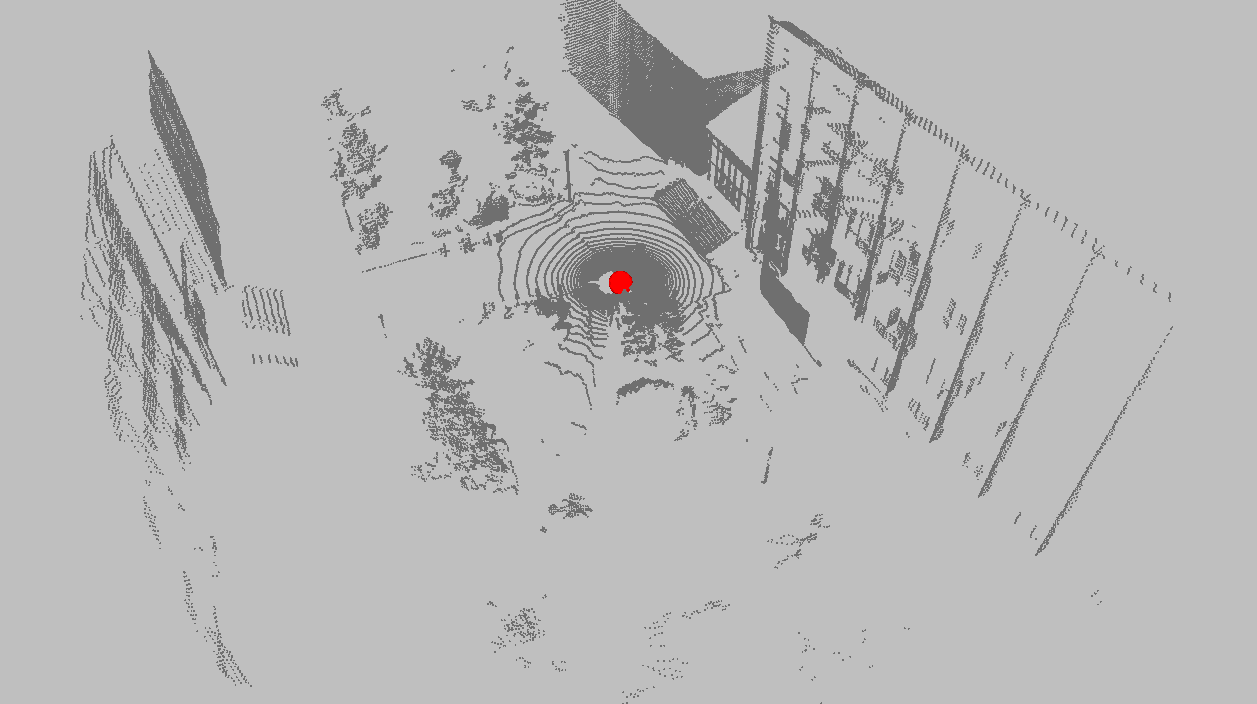
\includegraphics[width=0.47\linewidth]{img/chap_slam/pointcloud_building1.png}} \hspace{2mm}
    \subfloat[]{\label{fig:slam_pointcloud_building2}}{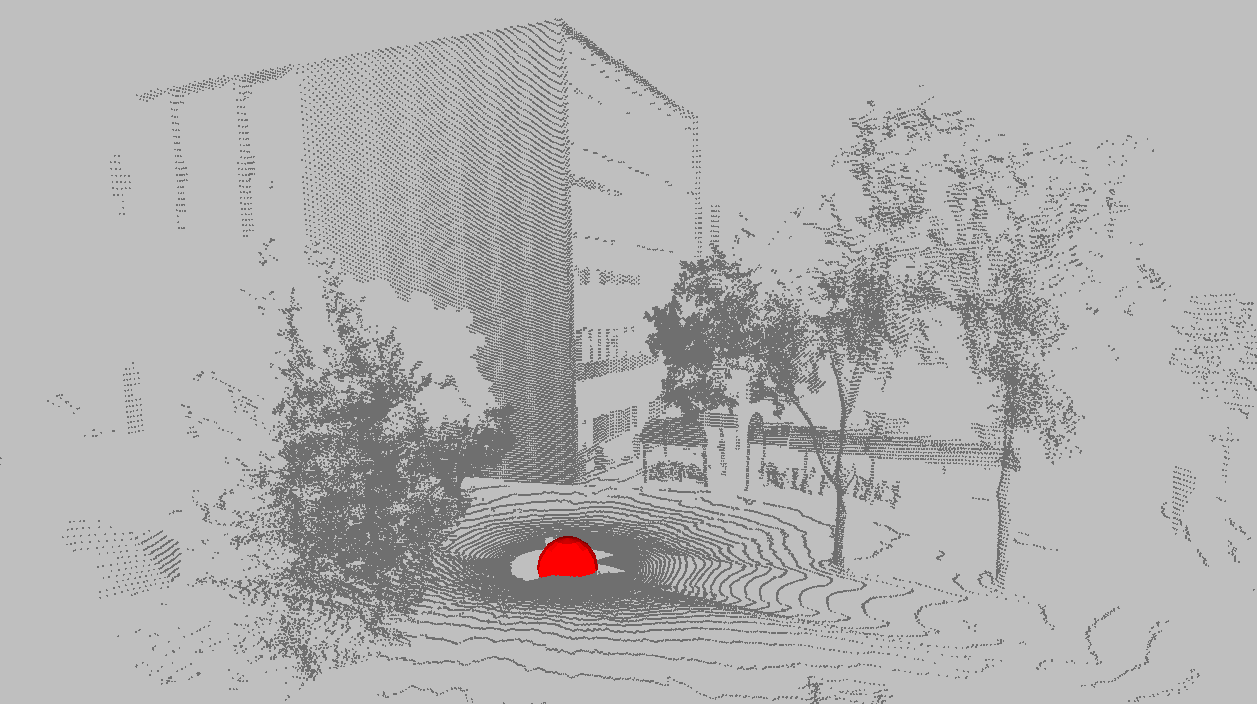
\includegraphics[width=0.47\linewidth]{img/chap_slam/pointcloud_building2.png}}
    \subfloat[]{\label{fig:slam_pointcloud_forest1}}{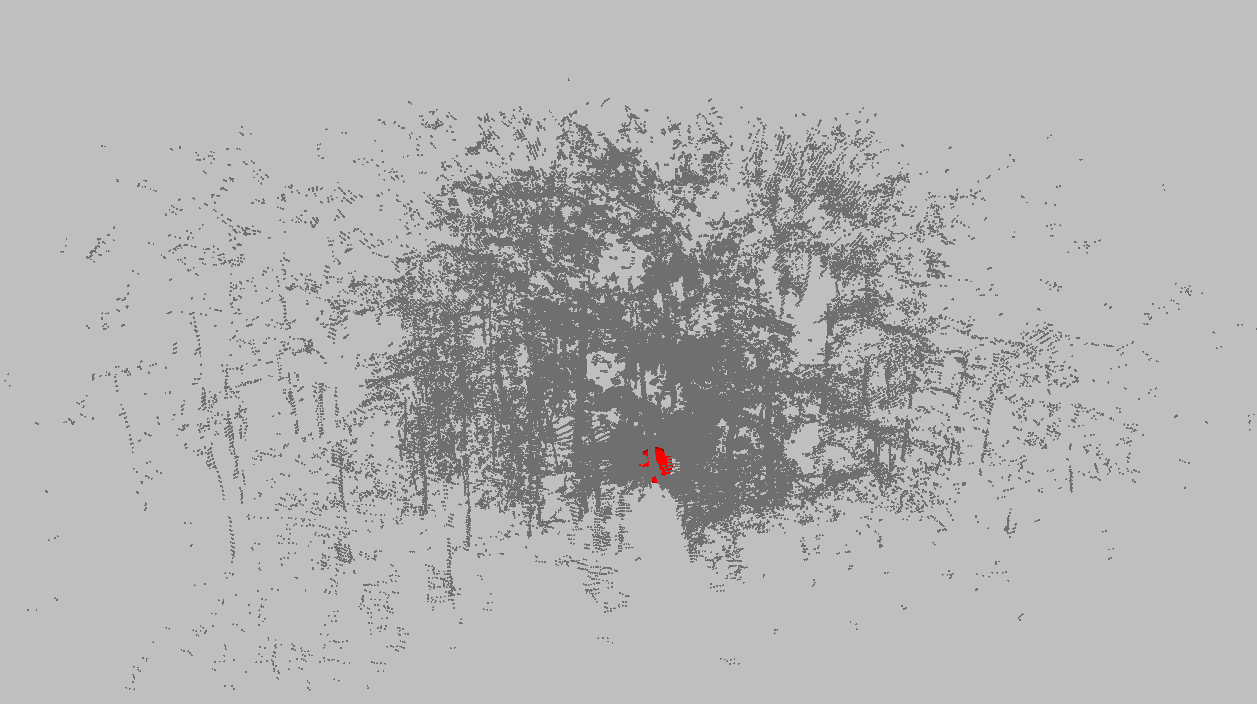
\includegraphics[width=0.47\linewidth]{img/chap_slam/pointcloud_forest1.png}} \hspace{2mm}
    \subfloat[]{\label{fig:slam_pointcloud_forest2}}{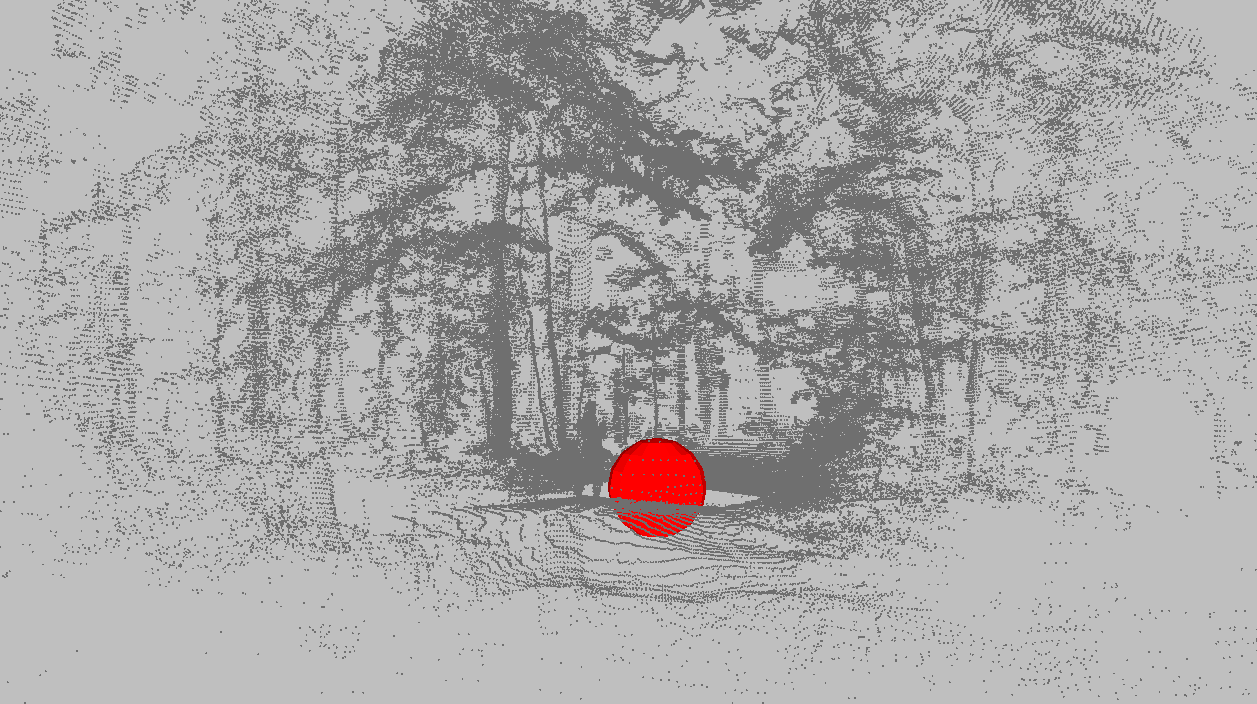
\includegraphics[width=0.47\linewidth]{img/chap_slam/pointcloud_forest2.png}}
    \subfloat[]{\label{fig:slam_pointcloud_velodyne1}}{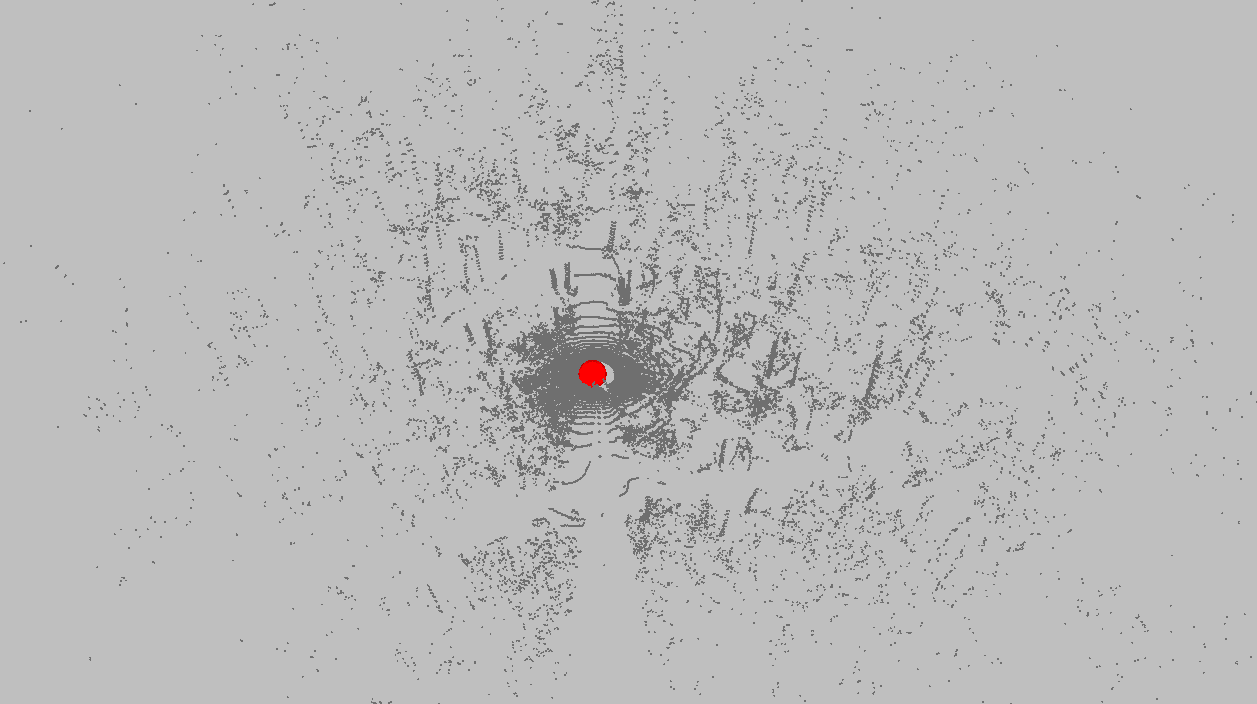
\includegraphics[width=0.47\linewidth]{img/chap_slam/pointcloud_velodyne1.png}} \hspace{2mm}
    \subfloat[]{\label{fig:slam_pointcloud_velodyne2}}{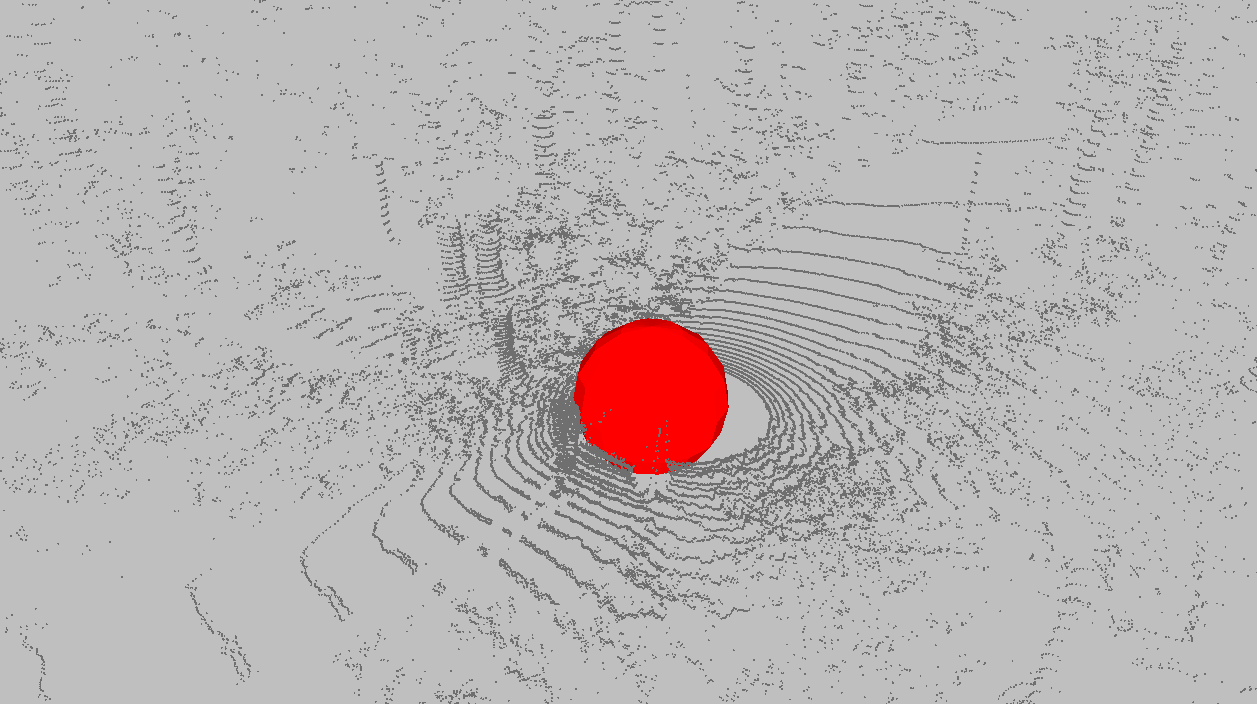
\includegraphics[width=0.47\linewidth]{img/chap_slam/pointcloud_velodyne2.png}}
    \caption[Examples of point clouds from our datasets viewed from different perspectives.]{Examples of point clouds from our datasets viewed from different perspectives. \protect\subref{fig:slam_pointcloud_building1} and \protect\subref{fig:slam_pointcloud_building2} show acquisition from the SICK in the structured environment. \protect\subref{fig:slam_pointcloud_forest1} and \protect\subref{fig:slam_pointcloud_forest2} also show point clouds from the SICK, but in the unstructured environment. Finally, \protect\subref{fig:slam_pointcloud_velodyne1} and \protect\subref{fig:slam_pointcloud_velodyne2} show the result of acquisition from the Velodyne in the unstructured environment. Robot position is represented by a red sphere with a \SI{1}{\meter} radius in each picture.}
    \label{fig:slam_pointclouds}
\end{figure}

